%!TEX encoding = UTF-8 Unicode

\section{ウェブインタフェースを介したHPCシステム利用環境}

\subsection{緒言}
前章では,本研究の関連研究について述べた.本章では,ウェブインタフェースを介したHPCシステム利用環境の提案手法について説明し,その実装を行う.はじめに,提案手法の概要を説明する.その後,実装の概要,具体的な実装の手順について説明する.\par

\subsection{従来手法}
従来のウェブインタフェースを介したHPCシステム利用環境について説明する.従来手法の模式図を図\ref{fig5}に示す.ウェブインタフェースはユーザとスケジューラのを直接結ぶ構成になっている.外部の認証用ディレクトリと連携してユーザ情報を管理することで,ウェブブラウザ上での利用空間の提供を行う.また,主要なスケジューラの抽象化を行うことで,統一的な操作環境を提供する.前章で述べたように,このシステム構成はシステムを改修する際にウェブインタフェース本体を改修する必要があるため,改修中に技術者の予期しない影響を与えてしまう可能性があり,保守性に問題がある.\par

\begin{figure}[tb]
    \centering
    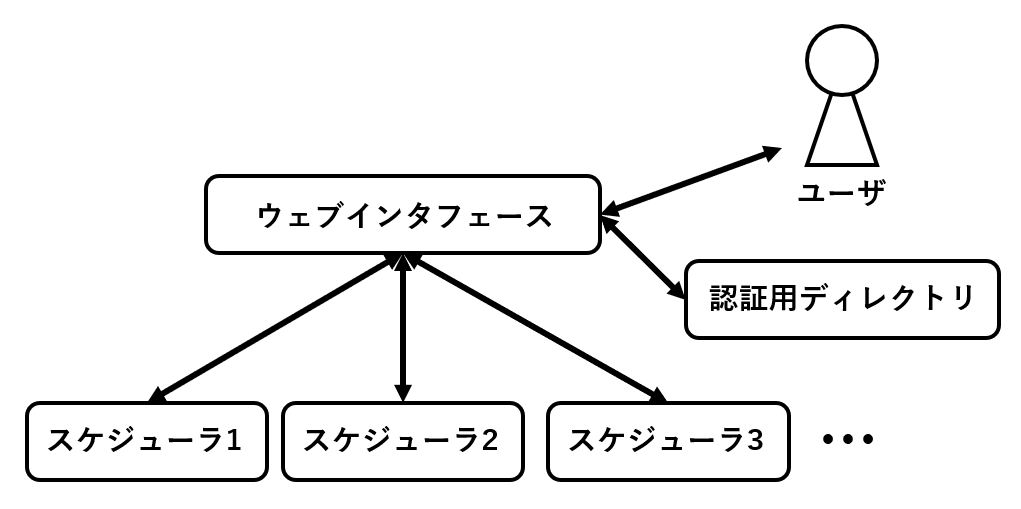
\includegraphics[width=100mm]{./fig/conventional_method.png}
    \caption{従来手法の模式図}
    \label{fig5}
\end{figure}

\subsection{提案手法}
本研究の目的は,HPC利用環境をウェブインタフェースに提供する機能(ウェブ機能)と,ジョブスケジューラ間の差異を抽象化する機能(スケジューラ抽象化機能)に切り分け,それぞれ独立に保守できる構成を実現することである.このために,本研究ではウェブ機能からは統一的にシステムを利用し,スケジューラ抽象化機能でシステム間の差異を埋める構成の利用環境を提案する.\par
この提案手法の模式図を図\ref{fig6}に示す.フロントエンドでは,ユーザはウェブ機能のみとやり取りを行い,ユーザ情報を管理する外部の認証用ディレクトリを用いて安全にHPC システムを利用することができる.バックエンドでは,ウェブ機能から得られた様々なスケジューラに対するリクエストをスケジューラ抽象化機能が受け取り,処理を行う.この実現のためには,ウェブ機能とスケジューラ抽象化機能を連携させる必要があることから,両者間に求められる情報のやり取りを整理し,適切な連携方法を検討する.\par

\begin{figure}[tb]
    \centering
    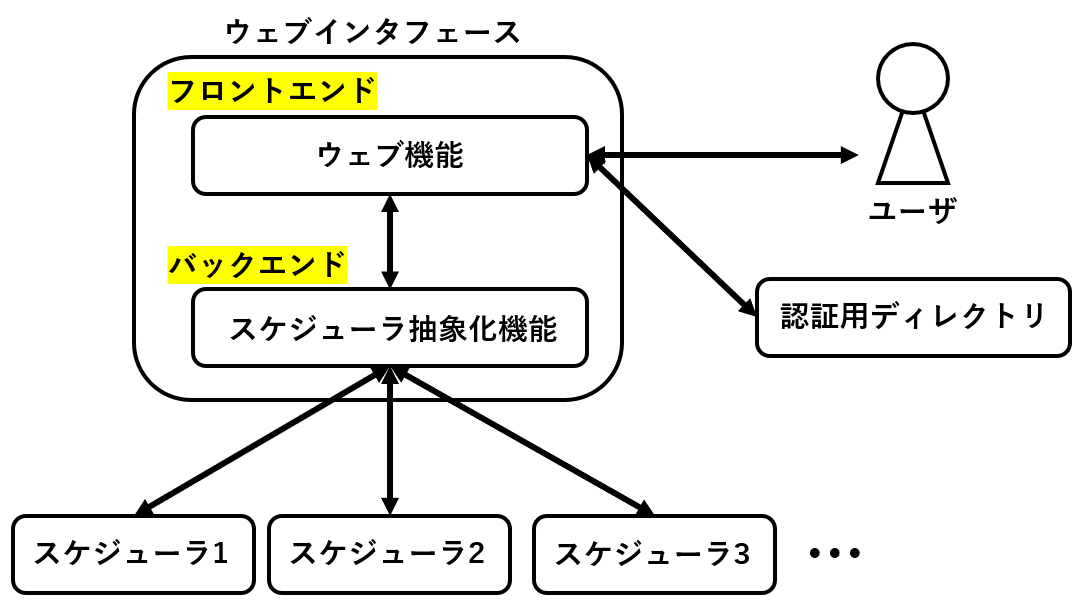
\includegraphics[width=100mm]{./fig/proposed_method.png}
    \caption{提案手法の模式図}
    \label{fig6}
\end{figure}

\subsection{実装}
\subsubsection{実装の概要}
ウェブ機能とスケジューラ抽象化機能をそれぞれ独立に実装し,連携させることでウェブインタフェースを介して様々なシステムを統一的に利用できる環境を実現する.そのために,ウェブ機能の基盤としてOOD,スケジューラ抽象化機能の基盤としてPSI/J\cite{cite5}と呼ばれるPythonライブラリを利用し,両者を組み合わせることで提案手法を実装する.\par
本研究では,東北大学のスーパーコンピュータ「AOBA」で運用されているジョブスケジューラ(NEC Network QueuingSystem V, NQSV) がOOD に対応していないという事実に着目して,NQSV をスケジューラ抽象化機能側に実装することと,それをウェブ機能側から利用できることを検証する.実装環境として,OOD用のホストサーバとスーパーコンピュータAOBAを模したHPCクラスタ(疑似AOBAクラスタ)を考える.模式図を図\ref{fig7}に示す.OOD用のホストサーバでは,OODの動作が保証されているUbuntu20.04 LSTをOSとして用いる.疑似AOBAクラスタは,マスターノードと二つのワーカーノードから構成される小規模なクラスタであり,AOBAと同様にNQSVがジョブスケジューラとして利用されている.疑似SOBSクラスタではQSVの動作確認が行われているCentOS7を用いる.OODはログイン時に認証機構を必要としており,dexとのOpeIDコネクトやShibboleth,CASなどの認証方法がある.本研究の実装では,公式が推奨しているDexとのOpenIDコネクトを用いてLDAP認証を行う.認証用ディレクトリであるLDAPサーバと連携して認証機構を設計する.\par

\begin{figure}[tb]
    \centering
    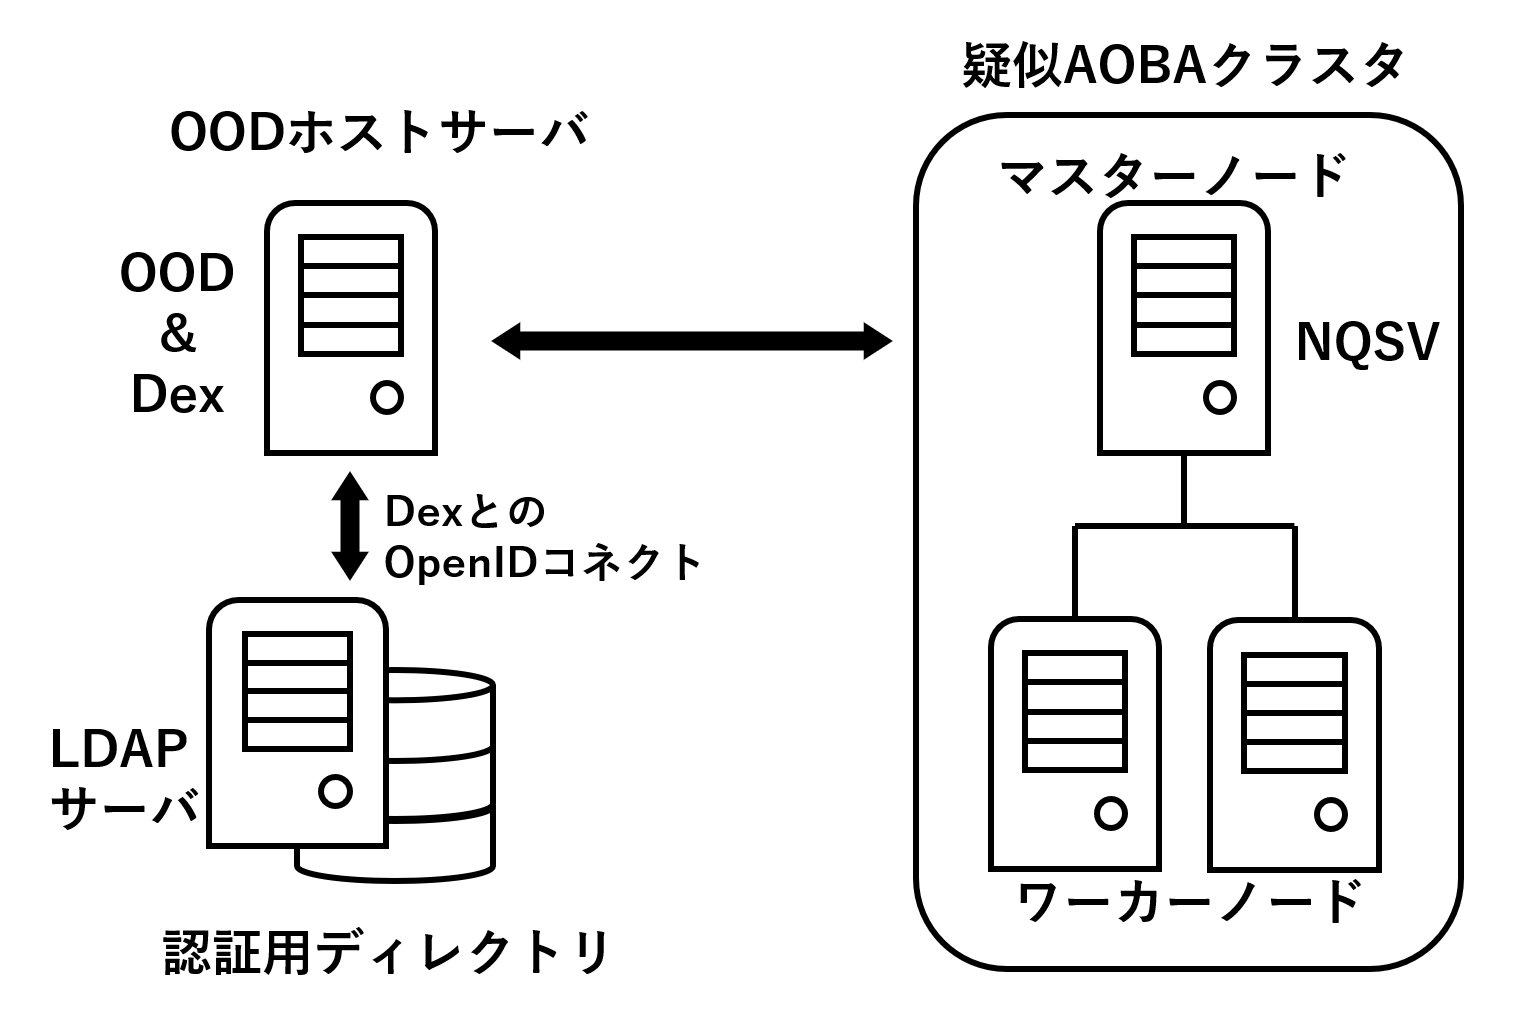
\includegraphics[width=100mm]{./fig/environment.png}
    \caption{実装環境}
    \label{fig7}
\end{figure}


\subsubsection{スケジューラ抽象化機能とNQSVの連携}
はじめに,スケジューラ抽象化機能とNQSVの連携を考える.スケジューラ抽象化機能の基板であるPSI/Jは,ジョブの情報を格納するJobクラスとジョブの投入や削除などのメソッドをスケジューラごとに再定義しているJobExecutorクラスにより構成されている.本研究では新たにNQSV用のJobExecutorクラスを作成し,ジョブの投入,削除,ジョブの状態確認を行うための三つのメソッドを実装する.
PSI/Jが対応している他のスケジューラ(Slurm,PBS Pro,LSF,Flux,Cobalt)はジョブの終了後にジョブの状態(COMPLETED,CANCELED,FAILED)をコマンドの出力結果から確認できる.しかし,NQSVではジョブの終了後にCOMPLETED,CANCELED,FAILEDの状態を確認できない.そのため,NQSVに対応するためには,ジョブの投入,ジョブの削除,および待機中のジョブの存在確認に基づいてジョブの状態をPSI/J側で把握する必要がある.この機能を実現するため,本研究の実装ではジョブが投入された後にジョブキューからジョブが無くなった際に,そのジョブの状態をCOMPLETEDに変更する.また,ジョブが削除された際には,そのジョブの状態をCANCELEDに変更する.それ以外にジョブキューの状態をコマンドを用いて定期的に確認し,出力結果に応じてQUEUEDあるいはACTIVEという状態にする.\par
具体的な実装をコード\ref{get_status_now}に示す.必要なライブラリのインポートや関数外の変数の宣言などは省略する.JobExecutorクラス内で定義されているget\_status\_nowメソッドはJobクラスのインスタンスを引数にとり,ジョブの状態を保持するJobStatusクラスを返り値に持つ.引数から受け取ったJobクラスのインスタンスからジョブのIDを抽出し,書くスケジューラごとに指定されているジョブの状態確認コマンドをジョブIDを指定して投げる.出力は行ごとにlinesに代入され,中身をforループでまわす.指定したIDのジョブがキューにない場合は「Batch Request: ジョブID does not exist on クラスタのホスト名.」という出力が帰ってくるため,この出力が取得され,cancel時に立つcancel\_fragが立っていればCANCELED状態にする.一方,この出力が取得され,cancel\_fragが立っていない場合は,キュー内部にジョブがないが,ジョブの削除が行われていないので,ジョブの状態はCOMPLETEDにする.また,ジョブの投入時に立つsubmit\_fragが立っていない場合はそもそもジョブの投入が成功していないので状態をFAILEDにする.なお,他のスケジューラではジョブ状態の詳細メッセージ出力される場合があるが,NQSVにはメッセージ出力機能がないためmessage変数はNoneとしている.\par
このようにPSI/J自身がジョブの状態を管理することにより,さらに広い範囲のジョブスケジューラに対応することができることから,ジョブスケジューラ抽象化機能の汎用性を高めることができたといえる.\par

\begin{lstlisting}[caption=ジョブの状態取得メソッド, label=dockerfile]
class NQSVJobExecutor(BatchSchedulerExecutor):
    def get_status_now(self, job: Job) -> Job.status:
        native_ids = ''.join(str(job.native_id))
        command = ['qstat', '-F', 'rid,stt', '-n', '-l', native_ids]
        out = subprocess.run(command, capture_output=True, text=True).stdout
        r = {}
        lines = iter(out.split('\n'))

        for line in lines:
            if not line:
                continue
            cols = line.split()

            if(len(cols) == 8 and self.cancel_frag):
                s = cols[2]
                native_id = ""
                for char in s:
                    if char.isdigit():
                        native_id += char
                state = JobState.CANCELED
                r[native_id] = JobStatus(state=state, message=None)
                return r[native_id]
            
            elif(len(cols) == 8 and not(self.cancel_frag)):
                s = cols[2]
                native_id = ""
                for char in s:
                    if char.isdigit():
                        native_id += char
                state = JobState.COMPLETED
                r[native_id] = JobStatus(state=state, message=None)
                return r[native_id]

            elif(not(self.submit_frag)):
                s = cols[2]
                native_id = ""
                for char in s:
                    if char.isdigit():
                        native_id += char
                state = JobState.FAILED
                r[native_id] = JobStatus(state=state, message=None)
                return r[native_id]
            
            else:
                assert len(cols) == 2
                match = re.search(r'\b(\d+)\b', cols[0])
                native_id = match.group(1) if match else None
                native_state = cols[1]
                state = self._get_state(native_state)
                msg = None
                r[native_id] = JobStatus(state=state, message=msg)
                return r[native_id]
    
\end{lstlisting}
\label{get_status_now}

\subsubsection{ウェブ機能とスケジューラ抽象化機能との連携}

\subsection{結言}